\documentclass[11pt,]{article}
\usepackage{lmodern}
\usepackage{amssymb,amsmath}
\usepackage{ifxetex,ifluatex}
\usepackage{fixltx2e} % provides \textsubscript
\ifnum 0\ifxetex 1\fi\ifluatex 1\fi=0 % if pdftex
  \usepackage[T1]{fontenc}
  \usepackage[utf8]{inputenc}
\else % if luatex or xelatex
  \ifxetex
    \usepackage{mathspec}
  \else
    \usepackage{fontspec}
  \fi
  \defaultfontfeatures{Ligatures=TeX,Scale=MatchLowercase}
\fi
% use upquote if available, for straight quotes in verbatim environments
\IfFileExists{upquote.sty}{\usepackage{upquote}}{}
% use microtype if available
\IfFileExists{microtype.sty}{%
\usepackage{microtype}
\UseMicrotypeSet[protrusion]{basicmath} % disable protrusion for tt fonts
}{}
\usepackage[margin=1.0in]{geometry}
\usepackage{hyperref}
\hypersetup{unicode=true,
            pdfborder={0 0 0},
            breaklinks=true}
\urlstyle{same}  % don't use monospace font for urls
\usepackage{graphicx,grffile}
\makeatletter
\def\maxwidth{\ifdim\Gin@nat@width>\linewidth\linewidth\else\Gin@nat@width\fi}
\def\maxheight{\ifdim\Gin@nat@height>\textheight\textheight\else\Gin@nat@height\fi}
\makeatother
% Scale images if necessary, so that they will not overflow the page
% margins by default, and it is still possible to overwrite the defaults
% using explicit options in \includegraphics[width, height, ...]{}
\setkeys{Gin}{width=\maxwidth,height=\maxheight,keepaspectratio}
\IfFileExists{parskip.sty}{%
\usepackage{parskip}
}{% else
\setlength{\parindent}{0pt}
\setlength{\parskip}{6pt plus 2pt minus 1pt}
}
\setlength{\emergencystretch}{3em}  % prevent overfull lines
\providecommand{\tightlist}{%
  \setlength{\itemsep}{0pt}\setlength{\parskip}{0pt}}
\setcounter{secnumdepth}{0}
% Redefines (sub)paragraphs to behave more like sections
\ifx\paragraph\undefined\else
\let\oldparagraph\paragraph
\renewcommand{\paragraph}[1]{\oldparagraph{#1}\mbox{}}
\fi
\ifx\subparagraph\undefined\else
\let\oldsubparagraph\subparagraph
\renewcommand{\subparagraph}[1]{\oldsubparagraph{#1}\mbox{}}
\fi

%%% Use protect on footnotes to avoid problems with footnotes in titles
\let\rmarkdownfootnote\footnote%
\def\footnote{\protect\rmarkdownfootnote}

%%% Change title format to be more compact
\usepackage{titling}

% Create subtitle command for use in maketitle
\providecommand{\subtitle}[1]{
  \posttitle{
    \begin{center}\large#1\end{center}
    }
}

\setlength{\droptitle}{-2em}

  \title{}
    \pretitle{\vspace{\droptitle}}
  \posttitle{}
    \author{}
    \preauthor{}\postauthor{}
    \date{}
    \predate{}\postdate{}
  
\usepackage{helvet} % Helvetica font
\renewcommand*\familydefault{\sfdefault} % Use the sans serif version of the font

%\usepackage{mathpazo} % Palatino font
%\renewcommand*\familydefault{\rmdefault} % Use the roman version of the font

\usepackage[T1]{fontenc}

\usepackage[none]{hyphenat}

\usepackage{setspace}
\doublespacing
\setlength{\parskip}{1em}

\usepackage{lineno}

\usepackage{pdfpages}

\begin{document}

\vspace*{10mm}

\hypertarget{reintroducing-mothur-10-years-later}{%
\section{Reintroducing mothur: 10 years
later}\label{reintroducing-mothur-10-years-later}}

\vspace{35mm}

Patrick D. Schloss\({^1}\)\({^\dagger}\)

\vspace{40mm}

\(\dagger\) To whom correspondence should be addressed:
\href{mailto:pschloss@umich.edu}{pschloss@umich.edu}

\(1\) Department of Microbiology and Immunology, University of Michigan,
Ann Arbor, MI 48109

\vspace{35mm}

\hypertarget{mini-review}{%
\subsubsection{Mini-review}\label{mini-review}}

\newpage
\linenumbers

\hypertarget{abstract}{%
\subsection{Abstract}\label{abstract}}

More than 10 years ago, we published the manuscript describing the
mothur software package in \emph{Applied and Environmental
Microbiology}. Our goal was to create a comprehensive package that
allowed users to analyze amplicon sequence data using the most robust
methods available. mothur has helped lead the community through the
ongoing sequencing revolution and continues to provide this service to
the microbial ecology community. Beyond its success and impact on the
field, mothur's development exposed a series of observations that are
generally translatable across science. Perhaps the observation that
stands out the most is that all science is done in the context of
prevailing ideas and available technologies. Although it is easy to
criticize choices that were made 10 years ago through a modern lens, if
we were to wait for all of the possible limitations to be solved before
proceeding, science would stall. Even preceding the development of
mothur, it was necessary to address the most important problems and work
backwards to other problems that limited access to robust sequence
analysis tools. At the same time, we strive to expand mothur's
capabilities in a data-driven manner to incorporate new ideas and
accommodate changes in data and desires of the research community. It
has been edifying to see the benefit that a simple set of tools can
bring to so many other researchers.

\newpage

Few scientists set out on a nearly two decade-long journey with a
specific goal in mind. Often we fail to start a scientific journey
because it looks too hard. Perhaps we get discouraged by all of the
things that could go wrong. Maybe we stray from the path because we find
something that is more interesting. Every scientist picks their own path
and takes their own forks in the road. From the outside, it may appear
to be a random walk. Nevertheless, these meanderings are common in
science.

Looking back on scientific journeys can be instructive to others who are
overwhelmed at the prospect of looking forward at their careers (1--5).
By no means is my scientific journey over, but since 2002 I have been on
a journey that I did not realize I was on. Now that the paper
introducing the mothur software package is ten years old and has become
the most cited paper published by \emph{Applied and Environmental
Microbiology} (7) (Figure 1), it is worth stepping back and using the
continued development of mothur as a story that has parallels to many
other research stories.

I fondly recall preparing a poster for the 2002 meeting of research
groups supported by the NSF-supported Microbial Observatories Program. I
wanted to triumphantly show that I had sequenced more than 600 16S rRNA
gene sequences from a single 0.5-g sample of Alaskan soil. This was
greater sequencing depth than anyone else had achieved for a single
sample. As I was preparing the poster, I walked into the office of Jo
Handelsman, my postdoctoral research advisor at the University of
Wisconsin, and laid out the outline for the poster. She asked if I could
add one of those ``curvy things'', a rarefaction curve, to show where I
was in sampling the community. Rarefaction curves and attempts to
estimate the taxonomic richness of soil had become popular because of
the impactful review by Jennifer Hughes and her colleagues (8). Their
seminal paper introduced the field to operational taxonomic units
(OTUs), rarefaction curves, and richness estimates. I do not recall
whether my poster had a rarefaction curve on it, but Jo's question and
that review article primed my career.

\textbf{\emph{Introducing DOTUR and friends.}} When Jo asked me to
generate a rarefaction curve for the poster, the request was not
trivial. How would I bin the sequences into OTUs? Hughes and her
colleagues did it manually and with fewer than 300 sequences. Although I
could possibly do that for my 600 sequences, my goal was to generate
1,000 sequences from the sample and to repeat that sampling effort with
other samples. I needed something that could be automated. Furthermore,
the software that Hughes used to build rarefaction curves, EstimateS
(4), required a series of tedious data formatting steps to perform the
analyses we were interested in performing. I had found my first problem.
How would I assign sequences to OTUs and use that data to estimate the
richness and diversity of a sample? The second problem would involve
comparing the abundance of OTUs found in one sample to another sample.
The solution to the first problem, DOTUR (Distance-based OTUs and
Richness), took us two years to develop (9). DOTUR did two things: given
a matrix quantifying the genetic distance between pairs of sequences, it
would cluster those sequences into OTUs for any distance threshold to
define the OTUs and then it would use the frequency of each OTU to
calculate a variety of alpha diversity metrics. The solutions to the
second problem would come from our work to develop software including
\(\int\)-LIBSHUFF (10), SONS (Shared OTUs and Similarity) (11), and
TreeClimber (12). Around the same time, Catherine Lozupone and Rob
Knight were developing their UniFrac tools to compare communities with a
phylogenetic rather than OTU-based approach (13, 14). With these tools,
the field of microbial ecology had a quantitative toolbox for describing
and comparing microbial communities. Along the way Jo and I would
demonstrate the utility of such tools for answering questions like how
many OTUs were there in that sample of Alaskan soil and how many
sequences were needed to sample each of those OTUs (15)? Where were we
in the global bacterial census (16)? How does the word usage of
\emph{Goodnight, Moon} compare to that of \emph{Portrait of a Lady} and
more importantly how is this relevant to microbial ecology (17)? Most
edifying were the more than 2,400 papers that used DOTUR, SONS,
TreeClimber, or \(\int\)-LIBSHUFF to facilitate their own research
questions (Web of Science, October 1, 2019). Had we waited to solve all
of the problems that plagued 16S rRNA gene sequencing, we would still be
waiting.

It is important to remember that we knew there were many problems with
16S rRNA gene sequencing. We knew there were biases from extractions and
amplification (18--23). We knew there were chimeras (24--27). We knew
that bacteria varied in their \emph{rrn} copy number. Generating a
distance matrix was a prerequisite to using my tools. This was not
trivial, but by cobbling together other tools it was possible. We would
assemble, trim and correct Sanger sequence reads using Chromas or STADEN
(28), align the sequences using ClustalW (29) or ARB (30), check for
chimeras using partial treeing or Bellerephon (27), and calculate a
pairwise distance matrix using DNADIST from the PHYLIP package (31). At
the time, we knew that we only had a loose concept of a species based on
these distances (32). We hoped that an OTU defined as a group of
sequences more than 97\% similar to each other would be a biologically
meaningful unit regardless of whether it fit our notion of a bacterial
species. At the time, I felt that the biggest problems that I could
solve were how to cluster the sequences into OTUs and how to use those
clusterings to test our hypotheses. The only tool available at the time
that automated the clustering step was FastGroup, which implemented an
approximation of the single linkage algorithm (33). The high cost of
sequencing was also an impediment to experimentation and analysis in
microbial ecology. It was rare for a study design to have experimental
replicates so that one could perform a statistical test to compare
treatment groups. For example, in our testing we frequently used a
dataset comparing Scottish soils from Alison McCaig and colleagues (34).
This dataset consisted of two experimental groups, each replicated three
times with 45 sequences per replicate. Although great focus has been
placed on the depth of sampling afforded by 454 and Illumina sequencing,
the true benefit of the modern sequencing platforms is the ability to
affordably sequence a large number of technical and biological
replicates. In my opinion, this expansion in the number of replicates
more than makes up for the potential limitations incurred by their
shorter read lenght. In spite of the many technical challenges, we had
excuses and heuristics to solve problems that served our needs. It is
telling that a recent review of ``best practices'' in generating and
analyzing 16S rRNA gene sequences shows that we still have not solved
many of these issues and that we have, of course, identified additional
problems (35).

As we developed these tools, I found a unique niche in microbiology. My
undergraduate and graduate training as a biological engineer prepared me
to think about research questions from a systems perspective, to think
quantitatively, and to understand the value of using computer programs
to help solve problems. As an undergraduate student, I learned the
Pascal programming language and promptly forgot much of it. Although it
was a good language for teaching programming concepts, it did not catch
on outside of the classroom. Later, I learned MATLAB. Because it was an
expensive commercial programming environment and never caught on with
biologists, I also forgot much of it. Even if I forgot the programming
syntax of these languages, what learning these languages taught me was
the logic and structure of programming. As a postdoc, I would use this
background to learn the Perl programming language to better understand
how LIBSHUFF (i.e.~LIBrary SHUFFle), a tool for comparing the structure
of two communities, worked since it was written in Perl (36). After
writing my own version of LIBSHUFF, \(\int\)-LIBSHUFF, and seeing the
speed of the version written in C++ by my collaborator, Bret Larget, I
converted my Perl version of DOTUR into C++. At the time, the conversion
from Perl to C++ seemed like an academic exercise to learn a new
language. My Perl version of DOTUR took a minute or so to process the
final collection of 1,000 sequences and the C++ version took seconds.
Was that really such a big difference? In hindsight, as we now process
datasets with tens of millions of sequences, the decision to learn C++
was critical. The ability to pick up computer languages to solve
problems, enabled by my prior training in engineering, was a skill that
was virtually unheard of in microbiology. Today, researchers without the
ability to program are at a significant disadvantage (37).

\textbf{\emph{Introducing mothur.}} Shortly after DOTUR was published, I
received an email from Mitch Sogin, a scientist at the Marine Biology
Laboratory (Woods Hole, MA), who asked whether DOTUR could handle more
than a million sequences. Without answering his question, I asked where
he found a million sequences. Little did I know that his email would
represent another pivot in the development of these tools and my career.
His group would be the first to use 454 sequencing technology to
generate 16S rRNA gene sequences (38). Although DOTUR could assign
millions of sequences to OTUs, it was slow and required a significant
amount of RAM. As I left my postdoc to start my independent career
across the state from Sogin's lab at the University of Massachusetts in
Amherst, my plan was to rewrite DOTUR, SONS, \(\int\)-LIBSHUFF, and
TreeClimber for the new world of massively parallelized sequencing. The
new tool would become mothur.

Milling about at a poster session at the 2007 ASM General Meeting in
Toronto, I ran into Mitch who asked what my plans were for my new lab. I
told him that I wanted to make a tool like ARB, a powerful database tool
and phylogenetics package (30), but for microbial ecology analysis. His
retort was, ``You and what army?'' Up to that point, I had written every
line of code and been answering many emails from people asking for help.
He was right, I would need an army. It would be difficult, but I needed
to learn to let go and share the development process with someone else.
My ``army'' ended up being Sarah Westcott who has worked on the mothur
project from its inception. Today, mothur is nearly 200,000 lines of
code and Sarah has touched or written nearly every line of it. Beyond
writing and testing mothur's code base, she has become a conduit for
many who are trying to learn the tools of microbial ecology. She
patiently answers questions via email and on the package's discussion
forum (\url{https://forum.mothur.org}). The community and I are lucky
that Sarah has stayed with the project for more than a decade. To be
honest, such dependency on a single person makes the project brittle. In
hindsight, it would have been better to have developed mothur with more
of an ``army'' or team so that there is overlap in people's
understanding of how mothur works. Although a distributed team approach
might work in a software engineering firm, it is not practical in most
academic environments where there is limited funding. There are
certainly projects that make this work, but they are rare.

\textbf{\emph{Competition has been good and healthy.}} mothur has not
been developed in a vacuum and it does not have a monopoly within the
field. As indicated above, each of our decisions were made in the
historical context of the field and with constant pressure from others
developing their own tools for analyzing 16S rRNA gene sequence data.
Competition has been good for mothur and for the field.

From the beginning there have been online tools available at the
Ribosomal Database Project (RDP) (39), greengenes (40), and SILVA (41).
These allowed users a straightforward method of comparing their data to
those collected in a database. There are two primary downsides to these
tools. First, researchers running the online tool must pay the
computational expenses. When their hardware becomes outdated because it
is expensive to replace or maintain, processing times slow down.
Eventually this limitation would result in the termination of the
greengenes website. Second, these platforms provide a one-size-fits-all
analysis. These tools only allow a user to analyze 16S and in some cases
18S rRNA gene sequences. If a user sequences a different gene, then the
tool will not serve them. These observations resulted in two design
goals we have had with mothur: bringing the analysis to a user's
computer and separating a tool from a specific database. For example, we
commonly use a sequence alignment method that was originally developed
for greengenes (42), but use a SILVA-based reference alignment because
its superior quality (43, 44). In addition, we offer the \text{na\"ive}
Bayesian classifier developed by the RDP (45) and allow users to train
it to any database they want, including customized databases. In both
examples, users can align or classify non-rRNA gene sequence data. As
the bioinformatics tools have matured, both the RDP and SILVA offer
integrated pipelines for analyzing large datasets, albeit in
one-size-fits-all black box implementations.

With the growth in popularity of 16S rRNA gene sequencing there has
naturally been an expansion in the number of people developing tools to
analyze these data. Months after the paper describing mothur was
published, the paper describing QIIME was published (46). Over the past
10 years, many have attempted to create analogies comparing the two
programs: Pepsi vs Coke, Apple vs Windows, etc. It is never clear which
software is which brand and whether the comparisons are meant as a
complement or an insult. Regardless, both programs are very popular.
From my perspective, most of the differences are cosmetic
(\url{http://blog.mothur.org/2016/01/12/mothur-and-qiime/}). To me the
most meaningful difference between mothur and QIIME is the choice of
algorithms used to cluster sequences into OTUs. QIIME's advocacy for
open and closed-reference clustering and USEARCH or VSEARCH-based
\emph{de novo} clustering results in lower quality OTU assignments
relative to the \emph{de novo} clustering algorithms available within
mothur (47, 48). QIIME is set of wrapper scripts that help users to
transition data between independent packages. For example, with QIIME
(through version 1.9.1), it was even possible to run mothur through
QIIME. One can also run the \text{na\"ive} Bayesian classifier through
QIIME using the original code developed by the RDP. This caused great
frustration for many users because there were numerous software
dependencies that had to be installed. Although the QIIME developers
would go on to create virtual machines and use packaging tools to
simplify installation, these fixes required sophistication by users who
we knew struggled with the basics of navigating a command line. In
contrast, when a user runs mothur, they are running mothur. The
\text{na\"ive} Bayesian classifier code that is in mothur is a rewritten
version of the original code. When we rewrite someone's software we do
it with an eye to improving performance, access, and utility for non-16S
rRNA gene sequence data. For example, while 454 data was popular,
PyroNoise was an effective tool for denoising flowgram data (49).
Running the original code required a large Linux computer cluster and
knowledge of bash and Perl scripting. When we rewrote the code for
mothur, we made it accessible to people using any operating system with
a simple command interface (i.e.~trim.flows and shhh.flows). Our
approach requires significant developer effort, but saves considerable
user effort. As this benefit is multiplied across thousands of projects,
the savings to users has been considerable.

Beyond the large packages like mothur and QIIME, there has been
significant growth in standalone software tools for sequence curation
(e.g.~PyroNoise (49), PANDAseq (50), DADA2 (51)), chimera checking
(e.g.~UCHIME (52), ChimeraSlayer (53), Perseus (54)), and clustering
(e.g.~USEARCH (55), VSEARCH (56), Swarm (57)). Where possible and when
warranted, we have implemented many of these algorithms directly into
mothur. We have also used this diversity of methods to perform
head-to-head comparisons. Most notable is the area of clustering
algorithms where there have been a large number of algorithms developed
without an obvious method to objectively compare them (47, 48, 58, 59).
We applied an objective metric, the Matthew's Correlation Coefficient
(MCC), to evaluate numerous algorithms for clustering sequences into
OTUs. By performing this type of analysis, we were able to objectively
compare the algorithms, make recommendations to the field, and develop
new algorithms that outperformed the existing ones. Beyond evaluating
clustering algorithms, we have also evaluated methods of denoising
sequence data (60--62), assessed reference alignments (43, 44),
considered the importance of incorporating secondary structure
information in alignments (63), quantified the variation along the 16S
rRNA gene (44), and compared the statistical hypotheses tested by
commonly used tools (64). We have embraced the competition and diversity
of all methods being used to analyze amplicon data. This competition
forces us to identify the strengths and weaknesses of various methods so
that we can make recommendations to other researchers.

\textbf{\emph{mothur's core principles.}} As mothur has evolved with the
needs of the community, several core principles have emerged that direct
its development. First, mothur is a free, open source software package.
This has been critical in shaping the direction of mothur. We were
content for mothur to be an improved combination of DOTUR and SONS and
leverage existing tools for other steps. Yet, we quickly appreciated the
need for providing other steps in a sequence analysis pipeline to make
other tools more accessible. This decision was motivated by learning
that the code for greengenes's (42) and ARB/SILVA's aligners were not
open source or publicly available. Thus, we realized that such an
important functionality needed to be opened to the community (43). More
recently, the rejection of closed source, commercial tools can be seen
by the broader adoption of open source alternatives. This has been the
case with the rising popularity of VSEARCH over USEARCH within the
microbial ecology community (55, 56). Related to insuring that mothur's
code is open source, our second core principle is that we maintain
transparency to our users. Perhaps a user does not need to interrogate
every line of code, but they need to understand what is happening. Many
programs, including online workflows, encapsulate large elements of a
pipeline in a single command. In contrast, mothur forces the user to
specify each step of the pipeline. Although the former approach makes an
analysis easier for a beginner, it stifles users that need greater
control or understanding of the assumptions at each step. This control
over the pipeline has made it easier for researchers to customize
databases or adapt the pipeline to analyze non-16S rRNA gene sequence
data. Furthermore, we have provided ample instructional materials to
teach users how to implement robust pipelines and the theory behind each
step through the project's website (\url{https://www.mothur.org}).
Third, as I mentioned above, there has been a plethora of methods
proposed for generating amplicon sequence data, and curating, aligning,
checking for chimeras, classifying, and clustering the data. I am proud
of the data-driven approach we have taken to comparing these methods. A
description of a new method has limited value if it is not benchmarked
against other methods or control datasets. Through this core principle
and mothur's large reach into the community, we have helped to develop
standards in the analysis of 16S rRNA gene sequence data. Fourth, a
focus on enabling reproducibility has always been central to the
functionality of mothur. From the beginning, mothur's logfiles have
represented a transcript of the user's command and outputs. When it
became clear that researchers were not submitting their sequence data to
the Sequence Read Archive (SRA), we worked with the SRA developers to
create a mothur command (make.sra) that creates a package for submitting
sequence data through a special mothur portal. A more ambitious project
had its seed on April 1, 2013 when we announced a new ``function'' in
mothur: write.paper. The new command required that the user provide a
454 sff file and a journal title or impact factor. With this
information, mothur would generate a manuscript. This April Fools' Day
joke was poking fun at software that provided an analysis black box but
also at many users' sentiments that data analysis should be so cut and
dry. A few years later, we revisited this concept in the scope of
reproducibility. Why not explicitly script an analysis from downloading
data from the SRA through the rendering of a manuscript ready for
submission? This idea gave rise to the development of the Riffomonas
reproducible research tutorial series that enables researchers to write
their own version of write.paper (65). Perhaps the most important core
principle is that my research group uses mothur to analyze the data we
generate. This has proven critical as it again represents transparency
and hopefully provides confidence to mothur's users that we are not
making recommendations that we do not follow ourselves.

\textbf{\emph{Challenges of making open source count.}} Anyone can post
code to GitHub with a permissive license and claim to be an open source
software developer. Far more challenging is engaging the target
community to make contributions to that code. Frankly, we have struggled
to expand the number of people that make contributions to the mothur
code base. One challenge we face is that if we looked to others to
contribute code to mothur, they would need to know C++. Given the
paucity of microbiologists that can program in a compiled language like
C++, expecting that community to provide contributors who can write code
in a syntax that prizes execution efficiency over developer efficiency
was not realistic. In contrast, the QIIME development team could be more
distributed because their code base was primarily written in Python,
which prizes developer efficiency over execution efficiency. QIIME is a
series of wrappers that allow users to execute other developers' code,
making the use of a scripting language like Python attractive. Their
choices resulted in many tradeoffs that have impacted ease of
installation, usability, execution speed, and flexibility. If we were
offered funding to rewrite mothur, we would likely rewrite it as an R
package that leaned heavily on the R language's C++ interface packages.
Of course, such choices are always best in hindsight. When we started
developing mothur, the ability to interface between scripting languages
like R and Python and C++ code was not as well developed as it is today.
For example, the modern version of the Rcpp package was first released
in 2009 and its popularity was not immediate (66). The development of
mothur has been a product of the environment that it was created in.
Although these decisions have largely had positive outcomes, there have
been tradeoffs that caused us to sacrifice other goals.

Beyond contributing to the mothur code base, we sought out other ways to
include the community as developers. The paper describing mothur
included 15 co-authors, most of whom responded to a call to provide a
wiki page that described how they used an early version of mothur to
analyze a data set. Our vision was that authors might use the mothur
wiki to document reproducible workflows for papers using mothur but to
also provide instructional materials for others seeking to adapt mothur
for their uses (\url{https://www.mothur.org/wiki}). Unfortunately, once
the incentive of co-authorship was removed, researchers stopped
contributing their workflows to the wiki. Again, this vision and the
lack of the community's adoption of wikis as a mechanism for reporting
workflows was a product of the environment. Although wikis were popular
in the late 2000's, they lacked the ability to directly execute the
commands that researchers reported. Such technology would not be
possible until the creation of IPython notebooks (2011) and R markdown
(2012). Another problem with the wiki approach was that potential
contributors did not see the wiki as a community resource. I frequently
received emails from scientists telling me that there was a typo on a
specific page when the intention was that they could correct the typos
without my input. We have been more successful in soliciting input and
contributions from the user community through the mothur discussion
forum and GitHub-based issue tracker. As mothur has matured, we have
been dependent on the user community to use these resources to tell us
what features they would like to see included in mothur and where the
documentation is confusing or incomplete
(\url{https://forum.mothur.org}). Often we can count on people not
directly affiliated with mothur to provide instruction and their own
experience to other users on the forum. We are constantly trying to
recruit our ``army'' and are happy to take any contributions we can.
Whether the contributions are to the code base, discussion forum, or
suggestions for new tools, these contributions have been invaluable to
the growth and popularity of mothur.

\textbf{\emph{Failed experiments.}} If we never failed, we would not be
trying hard enough. Over the past decade we have tried a number of
experiments to improve the usability and utility of mothur. One of our
first experiments was to use mothur to generate standard vector graphic
(SVG)-formatted files of heatmaps and Venn diagrams depicting the
overlap between microbial communities. Such visuals were helpful for
exploring data; however, I quickly realized that I would never put a
mothur-generated figure into a manuscript I wrote. Such visuals require
far too much customization to be publication-quality. Although QIIME has
incorporated visualization tools through the Emperor package (67), the
challenge of users taking default values has downsides, especially when
those defaults do not follow good data visualization principles. For
example, ordinations with black backgrounds and 3-D ordinations in a 2-D
medium now litter the literature. Instead, we have encouraged users to
use R packages to visualize mothur-generated results using the minimalR
instructional materials that I have developed
(\url{http://www.riffomonas.org/minimalR/}). A second experiment was the
creation of a graphical user interface (GUI) for running mothur. Forcing
users to interact with mothur through the command line has been a
significant hurdle for many (Figure 3). Unfortunately, the development
effort required to create and maintain a GUI is significant and there is
limited funding for such efforts. The newest version of QIIME (starting
with version 2.0.0) has emphasized interaction with the tools through a
GUI (68) and the related QIITA project offers a web-based GUI (69). It
remains to be seen how this experiment will go. Another downside of
using a GUI is that there is a risk that reproducibility will suffer if
users do not have a mechanism to document their mouse clicks. A
significant downside for web interfaces is the frequent inability to
document or return to old versions of software and databases. As was
experienced with greengenes, if the website is terminated, reproducing
old analyses becomes impossible. In mothur, documentation of commands
and parameter values is explicit in users can provide a file with a list
of commands and the software returns a logfile with all commands and
output recorded. Given the heightened focus on reproducibility in recent
years, we have extended significant effort in developing instructional
materials teaching users how to organize, document, and execute
reproducible pipelines that allow a user to go from raw sequence data to
a compiled manuscript (65, 70). A final example of a failed experiment
was a collaboration with programmers through Google Summer of Code to
develop commands in mothur that ran the random forest and SVM machine
learning algorithms. Similar to the challenges of developing attractive
visuals, fitting the algorithms' hyperparameters, testing, and deploying
the resulting models require a significant amount of customization.
Furthermore, machine learning is an active area of research where
methods are still being developed and improved. Thankfully, there are
numerous R and Python packages that do a better job of developing these
models (71, 72). In each of our ``failed'' experiments, the real
problems were straying from what mothur does well and failing to grasp
what we really wanted the innovation to do.

\textbf{\emph{The future.}} I will continue to develop mothur for as
long as other researchers find it useful. One challenge of such a plan
is maintaining the funding to support its development. The development
of mothur was initially enabled by a subcontract from a Sloan Foundation
grant to Mitch Sogin to support his VAMPS (Visualization and Analysis of
Microbial Population Structures) initiative. We used that seed funding
to secure an NSF grant and then a grant from NIH for tool development as
part of their Human Microbiome Project. Since that project expired in
2013, we have not had funding to specifically support mothur's
development. I have been fortunate to have start-up and discretionary
funds generated from other projects to help support mothur. Although
there is funding for new tools, there appears to be little appetite by
funders to support existing tools. Emblematic of this was the NIH
program, Big Data To Knowledge (BD2K), which solicited proposals through
the program announcement ``Extended Development, Hardening and
Dissemination of Technologies in Biomedical Computing, Informatics and
Big Data Science (PA-14-156)''. This opportunity appeared perfect,
except that the National Institute of Allergy and Infectious Diseases
(NIAID), the primary supporter of microbiome research at NIH, did not
participate in the announcement. Tools like mothur are clearly
successful, but need funding mechanisms to continue to mature and
support the needs of the research community.

As with anything in science, methods become \text{pass\'e}. When we
first developed mothur, T-RFLP and DGGE were still commonly used. Today
it would be hard to argue that data from those methods meaningfully
advance a study relative to what one could get using 16S rRNA gene
sequence data. Looking forward, many want to claim that amplicon
sequencing is today's DGGE. They claim that researchers should instead
move on to shotgun metagenomic sequencing. It is important to note that
the two methods answer fundamentally different questions. 16S rRNA gene
sequence data describes the taxonomic composition, while metagenomic
sequence data tells a researcher about the functional potential and
genetic diversity of a community. Both tools provide important
information, but they cannot easily replace each other. Although
metagenomic data does provide highly resolved taxonomic information, its
practical limit of detection is at least an order of magnitude higher
than that of amplicon data. For example, we analyzed 10,000 16S rRNA
sequences from each of about 500 subjects (73). We can think of this as
representing about 1,000,000 genome equivalents (10,000 16S rRNA
genes/subject x 500 subjects / 5 16S rRNA gene sequences/genome).
Assuming a genome is 4 Mbp, this would represent a sequencing depth of 4
Tbp. Although such a sequencing effort is technically possible, the cost
of such an endeavor would be considerable and unlikely to be pursued by
most researchers. We estimate that generating and sequencing the
libraries at the University of Michigan sequencing core would cost
approximately \$150 per library. The parallel 16S rRNA gene sequences
data would cost approximately \$8 per library. Furthermore, analyzing
such a large dataset with an approach that captures the full genetic
diversity of the community would be financially and technically
prohibitive. Going forward, sequencing technologies will continue to
evolve to capture longer and more high quality data and there will
always be a need for characterizing the taxonomic diversity of microbial
communities. With this in mind, there will always be a place for tools
like mothur that can analyze amplicon sequence data.

Of course this does not mean that such tools will remain static. We see
three key areas that we will continue to help the field to move forward.
First, just as we adapted through the transitions from Sanger to 454 to
MiSeq and PacBio sequencing platforms (60--62), we must learn whether
data from Oxford Nanopore and other developing sequencing technologies
can be an alternative sequencing approach that generates sequence data
that is the same quality as existing approaches; thus far, the approach
has significant shortcomings for sequencing 16S rRNA gene sequences
(74). As with the earlier platforms, we must better understand its error
profile so that sequencing errors can be corrected. We have learned that
moving forward requires that we maintain or improve sequence quality. No
doubt, datasets and read lengths will improve, but these advances should
not be made at the cost of data quality. Second, with these
improvements, we will need to continue to improve our algorithms. We
have already seen that attempts to use low quality MiSeq and HiSeq data
caused computational problems leading to the creation of open and closed
reference clustering methods, which attempted to circumvent those
problems (75, 76). Unfortunately, comparative analyses showed that these
methods fail relative to \emph{de novo} clustering methods (47, 48).
More work is needed to improve reference-based clustering methods so
that larger datasets can be analyzed without sacrificing the quality of
OTU assignments. Finally, there are ongoing controversies that need
further exploration. These include the validity and utility of amplicon
sequence variants (77), the wisdom of removing low frequency sequences
(78), and methods of identifying and removing contaminant 16S rRNA gene
sequences (79, 80). With each of these areas of development, the broader
community can count on our same data-driven approach to answer these
questions. It is common for researchers to comment that they pick a
specific method or deviate from a suggestion because they ``like how the
data look''. When pressed for an objective definition of how they know
the data look ``right'', they go quiet. Through the use of data where we
actually know what looks right and objective metrics of quality, we will
continue to base recommendations on data rather than a gut feeling.

\textbf{\emph{Conclusion.}} In the paper announcing mothur, we commented
that the relationship between 16S rRNA gene sequencing and analysis is
very much like the Red Queen in Lewis Carroll's book, \emph{Through the
Looking-Glass}. Although some disagreed with this analogy (81), I still
feel it is apt. The sequencing technology and rapacious appetite of
researchers continues to race on. At the same time, bioinformatics tools
must adapt to facilitate our research. I am confident that mothur will
be up to this exciting challenge. Beyond its utility for analyzing
amplicon sequence data, mothur's history provides lessons that are
helpful for other projects that hope to develop a long historical arc.
First, mothur is a product of its time. We have always sought to solve a
current need to the best of our ability with the tools we had at the
time. There are certainly caveats to any analysis of 16S rRNA gene
sequence data, but if we had waited until those caveats were resolved,
the field never would have progressed. Similarly, we made design choices
that we probably would not have made had we started the project today.
Second, as we have developed mothur, we have attempted to do so in a
data-driven approach where we compare multiple methods. It has not
merely been enough to propose a new method: we must show that it
meaningfully advances the field. Third, through our failures and
successes we have learned to focus on what mothur is good at and create
products separate from mothur when distinct needs arise. For example, we
have learned that mothur should not have a graphical interface or data
visualization tool. Instead, we provide instructional materials to teach
users how to use the command line interface and other computational
skills like programming in R for data visualization. Finally, mothur was
born out of a need for automating the analysis of large 16S rRNA gene
sequence datasets. It has been refreshing to see the computational
skills of the microbial ecology field grow over the past two decades.
Looking ahead, we must all take stock of the challenges we face in
microbial ecology and how our individual skills and interests can
address these challenges to turn them into opportunities.

\hypertarget{acknowledgements}{%
\subsection{Acknowledgements}\label{acknowledgements}}

The development of mothur would not be possible without the
contributions of its many supporters, developers, and users. Although
not a complete list, I would be remiss if I did not express my gratitude
to Sarah Westcott and the other members of my research group, Jo
Handelsman, Mitch Sogin, Susan Huse, Sarah Highlander, Vincent Young,
Lita Proctor, Kendra Maas, and Marcy Balunas for their unique
contributions to the continued development of mothur.

\newpage

\hypertarget{references}{%
\subsection{References}\label{references}}

\hypertarget{refs}{}
\leavevmode\hypertarget{ref-Lenski2017}{}%
1. \textbf{Lenski RE}. 2017. Experimental evolution and the dynamics of
adaptation and genome evolution in microbial populations. The ISME
Journal \textbf{11}:2181--2194.
doi:\href{https://doi.org/10.1038/ismej.2017.69}{10.1038/ismej.2017.69}.

\leavevmode\hypertarget{ref-Smith2018}{}%
2. \textbf{Smith DK}. 2018. From fundamental supramolecular chemistry to
self-assembled nanomaterials and medicines and back again how sam
inspired SAMul. Chemical Communications \textbf{54}:4743--4760.
doi:\href{https://doi.org/10.1039/c8cc01753k}{10.1039/c8cc01753k}.

\leavevmode\hypertarget{ref-Barbour2019}{}%
3. \textbf{Barbour AG}, \textbf{Benach JL}. 2019. Discovery of the lyme
disease agent. mBio \textbf{10}:e02166--19.
doi:\href{https://doi.org/10.1128/mbio.02166-19}{10.1128/mbio.02166-19}.

\leavevmode\hypertarget{ref-Colwell2014}{}%
4. \textbf{Colwell RK}, \textbf{Elsensohn JE}. 2014. EstimateS turns 20:
Statistical estimation of species richness and shared species from
samples, with non-parametric extrapolation. Ecography
\textbf{37}:609--613.
doi:\href{https://doi.org/10.1111/ecog.00814}{10.1111/ecog.00814}.

\leavevmode\hypertarget{ref-Glckner2017}{}%
5. \textbf{Glöckner FO}, \textbf{Yilmaz P}, \textbf{Quast C},
\textbf{Gerken J}, \textbf{Beccati A}, \textbf{Ciuprina A},
\textbf{Bruns G}, \textbf{Yarza P}, \textbf{Peplies J}, \textbf{Westram
R}, \textbf{Ludwig W}. 2017. 25 years of serving the community with
ribosomal RNA gene reference databases and tools. Journal of
Biotechnology \textbf{261}:169--176.
doi:\href{https://doi.org/10.1016/j.jbiotec.2017.06.1198}{10.1016/j.jbiotec.2017.06.1198}.

\leavevmode\hypertarget{ref-Casadevall2015}{}%
6. \textbf{Casadevall A}, \textbf{Fang FC}. 2015. (A)Historical science.
Infection and Immunity \textbf{83}:4460--4464.
doi:\href{https://doi.org/10.1128/iai.00921-15}{10.1128/iai.00921-15}.

\leavevmode\hypertarget{ref-Schloss2009a}{}%
7. \textbf{Schloss PD}, \textbf{Westcott SL}, \textbf{Ryabin T},
\textbf{Hall JR}, \textbf{Hartmann M}, \textbf{Hollister EB},
\textbf{Lesniewski RA}, \textbf{Oakley BB}, \textbf{Parks DH},
\textbf{Robinson CJ}, \textbf{Sahl JW}, \textbf{Stres B},
\textbf{Thallinger GG}, \textbf{Horn DJV}, \textbf{Weber CF}. 2009.
Introducing mothur: Open-source, platform-independent,
community-supported software for describing and comparing microbial
communities. Applied and Environmental Microbiology
\textbf{75}:7537--7541.
doi:\href{https://doi.org/10.1128/aem.01541-09}{10.1128/aem.01541-09}.

\leavevmode\hypertarget{ref-Hughes2001}{}%
8. \textbf{Hughes JB}, \textbf{Hellmann JJ}, \textbf{Ricketts TH},
\textbf{Bohannan BJM}. 2001. Counting the uncountable: Statistical
approaches to estimating microbial diversity. Applied and Environmental
Microbiology \textbf{67}:4399--4406.
doi:\href{https://doi.org/10.1128/aem.67.10.4399-4406.2001}{10.1128/aem.67.10.4399-4406.2001}.

\leavevmode\hypertarget{ref-Schloss2005}{}%
9. \textbf{Schloss PD}, \textbf{Handelsman J}. 2005. Introducing DOTUR,
a computer program for defining operational taxonomic units and
estimating species richness. Applied and Environmental Microbiology
\textbf{71}:1501--1506.
doi:\href{https://doi.org/10.1128/aem.71.3.1501-1506.2005}{10.1128/aem.71.3.1501-1506.2005}.

\leavevmode\hypertarget{ref-Schloss2004a}{}%
10. \textbf{Schloss PD}, \textbf{Larget BR}, \textbf{Handelsman J}.
2004. Integration of microbial ecology and statistics: A test to compare
gene libraries. Applied and Environmental Microbiology
\textbf{70}:5485--5492.
doi:\href{https://doi.org/10.1128/aem.70.9.5485-5492.2004}{10.1128/aem.70.9.5485-5492.2004}.

\leavevmode\hypertarget{ref-Schloss2006b}{}%
11. \textbf{Schloss PD}, \textbf{Handelsman J}. 2006. Introducing SONS,
a tool for operational taxonomic unit-based comparisons of microbial
community memberships and structures. Applied and Environmental
Microbiology \textbf{72}:6773--6779.
doi:\href{https://doi.org/10.1128/aem.00474-06}{10.1128/aem.00474-06}.

\leavevmode\hypertarget{ref-Schloss2006a}{}%
12. \textbf{Schloss PD}, \textbf{Handelsman J}. 2006. Introducing
TreeClimber, a test to compare microbial community structures. Applied
and Environmental Microbiology \textbf{72}:2379--2384.
doi:\href{https://doi.org/10.1128/aem.72.4.2379-2384.2006}{10.1128/aem.72.4.2379-2384.2006}.

\leavevmode\hypertarget{ref-Lozupone2005}{}%
13. \textbf{Lozupone C}, \textbf{Knight R}. 2005. UniFrac: A new
phylogenetic method for comparing microbial communities. Applied and
Environmental Microbiology \textbf{71}:8228--8235.
doi:\href{https://doi.org/10.1128/aem.71.12.8228-8235.2005}{10.1128/aem.71.12.8228-8235.2005}.

\leavevmode\hypertarget{ref-Lozupone2007}{}%
14. \textbf{Lozupone CA}, \textbf{Hamady M}, \textbf{Kelley ST},
\textbf{Knight R}. 2007. Quantitative and qualitative ~ diversity
measures lead to different insights into factors that structure
microbial communities. Applied and Environmental Microbiology
\textbf{73}:1576--1585.
doi:\href{https://doi.org/10.1128/aem.01996-06}{10.1128/aem.01996-06}.

\leavevmode\hypertarget{ref-Schloss2006c}{}%
15. \textbf{Schloss PD}, \textbf{Handelsman J}. 2006. Toward a census of
bacteria in soil. PLoS Computational Biology \textbf{2}:e92.
doi:\href{https://doi.org/10.1371/journal.pcbi.0020092}{10.1371/journal.pcbi.0020092}.

\leavevmode\hypertarget{ref-Schloss2004b}{}%
16. \textbf{Schloss PD}, \textbf{Handelsman J}. 2004. Status of the
microbial census. Microbiology and Molecular Biology Reviews
\textbf{68}:686--691.
doi:\href{https://doi.org/10.1128/mmbr.68.4.686-691.2004}{10.1128/mmbr.68.4.686-691.2004}.

\leavevmode\hypertarget{ref-Schloss2007}{}%
17. \textbf{Schloss PD}, \textbf{Handelsman J}. 2007. The last word:
Books as a statistical metaphor for microbial communities. Annual Review
of Microbiology \textbf{61}:23--34.

\leavevmode\hypertarget{ref-Zhou1996}{}%
18. \textbf{Zhou J}, \textbf{Bruns MA}, \textbf{Tiedje JM}. 1996. DNA
recovery from soils of diverse composition. Applied and Environmental
Microbiology \textbf{62}:316--322.

\leavevmode\hypertarget{ref-Suzuki1996}{}%
19. \textbf{Suzuki MT}, \textbf{Giovannoni SJ}. 1996. Bias caused by
template annealing in the amplification of mixtures of 16S rRNA genes by
pcr. Applied and Environmental Microbiology \textbf{62}:625--630.

\leavevmode\hypertarget{ref-Chandler1997}{}%
20. \textbf{Chandler DP}, \textbf{Fredrickson JK}, \textbf{Brockman FJ}.
1997. Effect of pcr template concentration on the composition and
distribution of total community 16S rDNA clone libraries. Molecular
Ecology \textbf{6}:475--482.

\leavevmode\hypertarget{ref-Polz1998}{}%
21. \textbf{Polz MF}, \textbf{Cavanaugh CM}. 1998. Bias in
template-to-product ratios in multitemplate pcr. Applied and
Environmental Microbiology \textbf{64}:3724--3730.

\leavevmode\hypertarget{ref-Wagner1994}{}%
22. \textbf{Wagner A}, \textbf{Blackstone N}, \textbf{Cartwright P},
\textbf{Dick M}, \textbf{Misof B}, \textbf{Snow P}, \textbf{Wagner GP},
\textbf{Bartels J}, \textbf{Murtha M}, \textbf{Pendleton J}. 1994.
Surveys of gene families using polymerase chain reaction: PCR selection
and pcr drift. Systematic Biology \textbf{43}:250--261.

\leavevmode\hypertarget{ref-Hansen1998}{}%
23. \textbf{Hansen MC}, \textbf{Tolker-Nielsen T}, \textbf{Givskov M},
\textbf{Molin S}. 1998. Biased 16S rDNA pcr amplification caused by
interference from dna flanking the template region. FEMS Microbiology
Ecology \textbf{26}:141--149.

\leavevmode\hypertarget{ref-Qiu2001}{}%
24. \textbf{Qiu X}, \textbf{Wu L}, \textbf{Huang H}, \textbf{McDonel
PE}, \textbf{Palumbo AV}, \textbf{Tiedje JM}, \textbf{Zhou J}. 2001.
Evaluation of pcr-generated chimeras, mutations, and heteroduplexes with
16S rRNA gene-based cloning. Applied and Environmental Microbiology
\textbf{67}:880--887.

\leavevmode\hypertarget{ref-Komatsoulis1997}{}%
25. \textbf{Komatsoulis GA}, \textbf{Waterman MS}. 1997. A new
computational method for detection of chimeric 16S rRNA artifacts
generated by pcr amplification from mixed bacterial populations. Applied
and Environmental Microbiology \textbf{63}:2338--2346.

\leavevmode\hypertarget{ref-Wang1997}{}%
26. \textbf{Wang G}, \textbf{Wang Y}. 1997. Frequency of formation of
chimeric molecules as a consequence of pcr coamplification of 16S rRNA
genes from mixed bacterial genomes. Applied and Environmental
Microbiology \textbf{63}:4645--4650.

\leavevmode\hypertarget{ref-Hugenholtz2003}{}%
27. \textbf{Hugenholtz P}, \textbf{Huber T}. 2003. Chimeric 16S rDNA
sequences of diverse origin are accumulating in the public databases.
International Journal of Systematic and Evolutionary Microbiology
\textbf{53}:289--293.

\leavevmode\hypertarget{ref-Bonfield1995}{}%
28. \textbf{Bonfield JK}, \textbf{Smith KF}, \textbf{Staden R}. 1995. A
new dna sequence assembly program. Nucleic Acids Research
\textbf{23}:4992--4999.

\leavevmode\hypertarget{ref-Thompson1994}{}%
29. \textbf{Thompson JD}, \textbf{Higgins DG}, \textbf{Gibson TJ}. 1994.
CLUSTAL w: Improving the sensitivity of progressive multiple sequence
alignment through sequence weighting, position-specific gap penalties
and weight matrix choice. Nucleic Acids Research \textbf{22}:4673--4680.
doi:\href{https://doi.org/10.1093/nar/22.22.4673}{10.1093/nar/22.22.4673}.

\leavevmode\hypertarget{ref-Ludwig2004}{}%
30. \textbf{Ludwig W}. 2004. ARB: A software environment for sequence
data. Nucleic Acids Research \textbf{32}:1363--1371.
doi:\href{https://doi.org/10.1093/nar/gkh293}{10.1093/nar/gkh293}.

\leavevmode\hypertarget{ref-Felsenstein1989}{}%
31. \textbf{Felsenstein J}. 1989. PHYLIP - phylogeny inference package.
Cladistics \textbf{5}:164--166.

\leavevmode\hypertarget{ref-Stackebrandt1994}{}%
32. \textbf{Stackebrandt E}, \textbf{Goebel BM}. 1994. Taxonomic note: A
place for DNA-DNA reassociation and 16S rRNA sequence analysis in the
present species definition in bacteriology. International Journal of
Systematic and Evolutionary Microbiology \textbf{44}:846--849.
doi:\href{https://doi.org/10.1099/00207713-44-4-846}{10.1099/00207713-44-4-846}.

\leavevmode\hypertarget{ref-Seguritan2001}{}%
33. \textbf{Seguritan V}, \textbf{Rohwer F}. 2001. FastGroup: A program
to dereplicate libraries of 16S rDNA sequences. BMC Bioinformatics
\textbf{2}:9.
doi:\href{https://doi.org/10.1186/1471-2105-2-9}{10.1186/1471-2105-2-9}.

\leavevmode\hypertarget{ref-McCaig1999}{}%
34. \textbf{McCaig AE}, \textbf{Glover LA}, \textbf{Prosser JI}. 1999.
Molecular analysis of bacterial community structure and diversity in
unimproved and improved upland grass pastures. Applied and Environmental
Microbiology \textbf{65}:1721--1730.

\leavevmode\hypertarget{ref-Pollock2018}{}%
35. \textbf{Pollock J}, \textbf{Glendinning L}, \textbf{Wisedchanwet T},
\textbf{Watson M}. 2018. The madness of microbiome: Attempting to find
consensus ``Best practice'' for 16S microbiome studies. Applied and
Environmental Microbiology \textbf{84}:e02627--17.
doi:\href{https://doi.org/10.1128/aem.02627-17}{10.1128/aem.02627-17}.

\leavevmode\hypertarget{ref-Singleton2001}{}%
36. \textbf{Singleton DR}, \textbf{Furlong MA}, \textbf{Rathbun SL},
\textbf{Whitman WB}. 2001. Quantitative comparisons of 16S rRNA gene
sequence libraries from environmental samples. Applied and Environmental
Microbiology \textbf{67}:4374--4376.
doi:\href{https://doi.org/10.1128/aem.67.9.4374-4376.2001}{10.1128/aem.67.9.4374-4376.2001}.

\leavevmode\hypertarget{ref-Carey2018}{}%
37. \textbf{Carey MA}, \textbf{Papin JA}. 2018. Ten simple rules for
biologists learning to program. PLOS Computational Biology
\textbf{14}:e1005871.
doi:\href{https://doi.org/10.1371/journal.pcbi.1005871}{10.1371/journal.pcbi.1005871}.

\leavevmode\hypertarget{ref-Sogin2006}{}%
38. \textbf{Sogin ML}, \textbf{Morrison HG}, \textbf{Huber JA},
\textbf{Welch DM}, \textbf{Huse SM}, \textbf{Neal PR}, \textbf{Arrieta
JM}, \textbf{Herndl GJ}. 2006. Microbial diversity in the deep sea and
the underexplored "rare biosphere". Proceedings of the National Academy
of Sciences \textbf{103}:12115--12120.
doi:\href{https://doi.org/10.1073/pnas.0605127103}{10.1073/pnas.0605127103}.

\leavevmode\hypertarget{ref-Cole2013}{}%
39. \textbf{Cole JR}, \textbf{Wang Q}, \textbf{Fish JA}, \textbf{Chai
B}, \textbf{McGarrell DM}, \textbf{Sun Y}, \textbf{Brown CT},
\textbf{Porras-Alfaro A}, \textbf{Kuske CR}, \textbf{Tiedje JM}. 2013.
Ribosomal database project: Data and tools for high throughput rRNA
analysis. Nucleic Acids Research \textbf{42}:D633--D642.
doi:\href{https://doi.org/10.1093/nar/gkt1244}{10.1093/nar/gkt1244}.

\leavevmode\hypertarget{ref-DeSantis2006a}{}%
40. \textbf{DeSantis TZ}, \textbf{Hugenholtz P}, \textbf{Larsen N},
\textbf{Rojas M}, \textbf{Brodie EL}, \textbf{Keller K}, \textbf{Huber
T}, \textbf{Dalevi D}, \textbf{Hu P}, \textbf{Andersen GL}. 2006.
Greengenes, a chimera-checked 16S rRNA gene database and workbench
compatible with ARB. Applied and Environmental Microbiology
\textbf{72}:5069--5072.
doi:\href{https://doi.org/10.1128/aem.03006-05}{10.1128/aem.03006-05}.

\leavevmode\hypertarget{ref-Yilmaz2013}{}%
41. \textbf{Yilmaz P}, \textbf{Parfrey LW}, \textbf{Yarza P},
\textbf{Gerken J}, \textbf{Pruesse E}, \textbf{Quast C}, \textbf{Schweer
T}, \textbf{Peplies J}, \textbf{Ludwig W}, \textbf{Glöckner FO}. 2013.
The SILVA and ``All-species living tree project (LTP)'' taxonomic
frameworks. Nucleic Acids Research \textbf{42}:D643--D648.
doi:\href{https://doi.org/10.1093/nar/gkt1209}{10.1093/nar/gkt1209}.

\leavevmode\hypertarget{ref-DeSantis2006b}{}%
42. \textbf{DeSantis TZ}, \textbf{Hugenholtz P}, \textbf{Keller K},
\textbf{Brodie EL}, \textbf{Larsen N}, \textbf{Piceno YM}, \textbf{Phan
R}, \textbf{Andersen GL}. 2006. NAST: A multiple sequence alignment
server for comparative analysis of 16S rRNA genes. Nucleic Acids
Research \textbf{34}:W394--W399.
doi:\href{https://doi.org/10.1093/nar/gkl244}{10.1093/nar/gkl244}.

\leavevmode\hypertarget{ref-Schloss2009b}{}%
43. \textbf{Schloss PD}. 2009. A high-throughput DNA sequence aligner
for microbial ecology studies. PLoS ONE \textbf{4}:e8230.
doi:\href{https://doi.org/10.1371/journal.pone.0008230}{10.1371/journal.pone.0008230}.

\leavevmode\hypertarget{ref-Schloss2010a}{}%
44. \textbf{Schloss PD}. 2010. The effects of alignment quality,
distance calculation method, sequence filtering, and region on the
analysis of 16S rRNA gene-based studies. PLoS Computational Biology
\textbf{6}:e1000844.
doi:\href{https://doi.org/10.1371/journal.pcbi.1000844}{10.1371/journal.pcbi.1000844}.

\leavevmode\hypertarget{ref-Wang2007}{}%
45. \textbf{Wang Q}, \textbf{Garrity GM}, \textbf{Tiedje JM},
\textbf{Cole JR}. 2007. Naive bayesian classifier for rapid assignment
of rRNA sequences into the new bacterial taxonomy. Applied and
Environmental Microbiology \textbf{73}:5261--5267.
doi:\href{https://doi.org/10.1128/aem.00062-07}{10.1128/aem.00062-07}.

\leavevmode\hypertarget{ref-Caporaso2010a}{}%
46. \textbf{Caporaso JG}, \textbf{Kuczynski J}, \textbf{Stombaugh J},
\textbf{Bittinger K}, \textbf{Bushman FD}, \textbf{Costello EK},
\textbf{Fierer N}, \textbf{Peña AG}, \textbf{Goodrich JK},
\textbf{Gordon JI}, \textbf{Huttley GA}, \textbf{Kelley ST},
\textbf{Knights D}, \textbf{Koenig JE}, \textbf{Ley RE},
\textbf{Lozupone CA}, \textbf{McDonald D}, \textbf{Muegge BD},
\textbf{Pirrung M}, \textbf{Reeder J}, \textbf{Sevinsky JR},
\textbf{Turnbaugh PJ}, \textbf{Walters WA}, \textbf{Widmann J},
\textbf{Yatsunenko T}, \textbf{Zaneveld J}, \textbf{Knight R}. 2010.
QIIME allows analysis of high-throughput community sequencing data.
Nature Methods \textbf{7}:335--336.
doi:\href{https://doi.org/10.1038/nmeth.f.303}{10.1038/nmeth.f.303}.

\leavevmode\hypertarget{ref-Westcott2015}{}%
47. \textbf{Westcott SL}, \textbf{Schloss PD}. 2015. De novo clustering
methods outperform reference-based methods for assigning 16S rRNA gene
sequences to operational taxonomic units. PeerJ \textbf{3}:e1487.
doi:\href{https://doi.org/10.7717/peerj.1487}{10.7717/peerj.1487}.

\leavevmode\hypertarget{ref-Westcott2017}{}%
48. \textbf{Westcott SL}, \textbf{Schloss PD}. 2017. OptiClust, an
improved method for assigning amplicon-based sequence data to
operational taxonomic units. mSphere \textbf{2}:e00073--17.
doi:\href{https://doi.org/10.1128/mspheredirect.00073-17}{10.1128/mspheredirect.00073-17}.

\leavevmode\hypertarget{ref-Quince2009}{}%
49. \textbf{Quince C}, \textbf{Lanzén A}, \textbf{Curtis TP},
\textbf{Davenport RJ}, \textbf{Hall N}, \textbf{Head IM}, \textbf{Read
LF}, \textbf{Sloan WT}. 2009. Accurate determination of microbial
diversity from 454 pyrosequencing data. Nature Methods
\textbf{6}:639--641.
doi:\href{https://doi.org/10.1038/nmeth.1361}{10.1038/nmeth.1361}.

\leavevmode\hypertarget{ref-Masella2012}{}%
50. \textbf{Masella AP}, \textbf{Bartram AK}, \textbf{Truszkowski JM},
\textbf{Brown DG}, \textbf{Neufeld JD}. 2012. PANDAseq: Paired-end
assembler for illumina sequences. BMC Bioinformatics \textbf{13}:31.
doi:\href{https://doi.org/10.1186/1471-2105-13-31}{10.1186/1471-2105-13-31}.

\leavevmode\hypertarget{ref-Callahan2016}{}%
51. \textbf{Callahan BJ}, \textbf{McMurdie PJ}, \textbf{Rosen MJ},
\textbf{Han AW}, \textbf{Johnson AJA}, \textbf{Holmes SP}. 2016. DADA2:
High-resolution sample inference from illumina amplicon data. Nature
Methods \textbf{13}:581--583.
doi:\href{https://doi.org/10.1038/nmeth.3869}{10.1038/nmeth.3869}.

\leavevmode\hypertarget{ref-Edgar2011}{}%
52. \textbf{Edgar RC}, \textbf{Haas BJ}, \textbf{Clemente JC},
\textbf{Quince C}, \textbf{Knight R}. 2011. UCHIME improves sensitivity
and speed of chimera detection. Bioinformatics \textbf{27}:2194--2200.
doi:\href{https://doi.org/10.1093/bioinformatics/btr381}{10.1093/bioinformatics/btr381}.

\leavevmode\hypertarget{ref-Haas2011}{}%
53. \textbf{Haas BJ}, \textbf{Gevers D}, \textbf{Earl AM},
\textbf{Feldgarden M}, \textbf{Ward DV}, \textbf{Giannoukos G},
\textbf{Ciulla D}, \textbf{Tabbaa D}, \textbf{Highlander SK},
\textbf{Sodergren E}, \textbf{Methe B}, \textbf{DeSantis TZ},
\textbf{Petrosino JF}, \textbf{Knight R}, \textbf{and BWB}. 2011.
Chimeric 16S rRNA sequence formation and detection in Sanger and
454-pyrosequenced PCR amplicons. Genome Research \textbf{21}:494--504.
doi:\href{https://doi.org/10.1101/gr.112730.110}{10.1101/gr.112730.110}.

\leavevmode\hypertarget{ref-Quince2011}{}%
54. \textbf{Quince C}, \textbf{Lanzen A}, \textbf{Davenport RJ},
\textbf{Turnbaugh PJ}. 2011. Removing noise from pyrosequenced
amplicons. BMC Bioinformatics \textbf{12}:38.
doi:\href{https://doi.org/10.1186/1471-2105-12-38}{10.1186/1471-2105-12-38}.

\leavevmode\hypertarget{ref-Edgar2010}{}%
55. \textbf{Edgar RC}. 2010. Search and clustering orders of magnitude
faster than BLAST. Bioinformatics \textbf{26}:2460--2461.
doi:\href{https://doi.org/10.1093/bioinformatics/btq461}{10.1093/bioinformatics/btq461}.

\leavevmode\hypertarget{ref-Rognes2016}{}%
56. \textbf{Rognes T}, \textbf{Flouri T}, \textbf{Nichols B},
\textbf{Quince C}, \textbf{Mahé F}. 2016. VSEARCH: A versatile open
source tool for metagenomics. PeerJ \textbf{4}:e2584.
doi:\href{https://doi.org/10.7717/peerj.2584}{10.7717/peerj.2584}.

\leavevmode\hypertarget{ref-Mah2015}{}%
57. \textbf{Mahé F}, \textbf{Rognes T}, \textbf{Quince C},
\textbf{Vargas C de}, \textbf{Dunthorn M}. 2015. Swarm v2:
Highly-scalable and high-resolution amplicon clustering. PeerJ
\textbf{3}:e1420.
doi:\href{https://doi.org/10.7717/peerj.1420}{10.7717/peerj.1420}.

\leavevmode\hypertarget{ref-Schloss2011a}{}%
58. \textbf{Schloss PD}, \textbf{Westcott SL}. 2011. Assessing and
improving methods used in operational taxonomic unit-based approaches
for 16S rRNA gene sequence analysis. Applied and Environmental
Microbiology \textbf{77}:3219--3226.
doi:\href{https://doi.org/10.1128/aem.02810-10}{10.1128/aem.02810-10}.

\leavevmode\hypertarget{ref-Schloss2016a}{}%
59. \textbf{Schloss PD}. 2016. Application of a database-independent
approach to assess the quality of operational taxonomic unit picking
methods. mSystems \textbf{1}:e00027--16.
doi:\href{https://doi.org/10.1128/msystems.00027-16}{10.1128/msystems.00027-16}.

\leavevmode\hypertarget{ref-Kozich2013}{}%
60. \textbf{Kozich JJ}, \textbf{Westcott SL}, \textbf{Baxter NT},
\textbf{Highlander SK}, \textbf{Schloss PD}. 2013. Development of a
dual-index sequencing strategy and curation pipeline for analyzing
amplicon sequence data on the MiSeq illumina sequencing platform.
Applied and Environmental Microbiology \textbf{79}:5112--5120.
doi:\href{https://doi.org/10.1128/aem.01043-13}{10.1128/aem.01043-13}.

\leavevmode\hypertarget{ref-Schloss2011b}{}%
61. \textbf{Schloss PD}, \textbf{Gevers D}, \textbf{Westcott SL}. 2011.
Reducing the effects of PCR amplification and sequencing artifacts on
16S rRNA-based studies. PLoS ONE \textbf{6}:e27310.
doi:\href{https://doi.org/10.1371/journal.pone.0027310}{10.1371/journal.pone.0027310}.

\leavevmode\hypertarget{ref-Schloss2016b}{}%
62. \textbf{Schloss PD}, \textbf{Jenior ML}, \textbf{Koumpouras CC},
\textbf{Westcott SL}, \textbf{Highlander SK}. 2016. Sequencing 16S rRNA
gene fragments using the PacBio SMRT DNA sequencing system. PeerJ
\textbf{4}:e1869.
doi:\href{https://doi.org/10.7717/peerj.1869}{10.7717/peerj.1869}.

\leavevmode\hypertarget{ref-Schloss2012a}{}%
63. \textbf{Schloss PD}. 2012. Secondary structure improves OTU
assignments of 16S rRNA gene sequences. The ISME Journal
\textbf{7}:457--460.
doi:\href{https://doi.org/10.1038/ismej.2012.102}{10.1038/ismej.2012.102}.

\leavevmode\hypertarget{ref-Schloss2008}{}%
64. \textbf{Schloss PD}. 2008. Evaluating different approaches that test
whether microbial communities have the same structure. The ISME Journal
\textbf{2}:265--275.
doi:\href{https://doi.org/10.1038/ismej.2008.5}{10.1038/ismej.2008.5}.

\leavevmode\hypertarget{ref-Schloss2018a}{}%
65. \textbf{Schloss PD}. 2018. The riffomonas reproducible research
tutorial series. Journal of Open Source Education \textbf{1}:13.
doi:\href{https://doi.org/10.21105/jose.00013}{10.21105/jose.00013}.

\leavevmode\hypertarget{ref-Eddelbuettel2011}{}%
66. \textbf{Eddelbuettel D}, \textbf{François R}. 2011. Rcpp: Seamless R
and C++ integration. Journal of Statistical Software \textbf{40}:1--18.
doi:\href{https://doi.org/10.18637/jss.v040.i08}{10.18637/jss.v040.i08}.

\leavevmode\hypertarget{ref-VzquezBaeza2013}{}%
67. \textbf{Vázquez-Baeza Y}, \textbf{Pirrung M}, \textbf{Gonzalez A},
\textbf{Knight R}. 2013. EMPeror: A tool for visualizing high-throughput
microbial community data. GigaScience \textbf{2}:16.
doi:\href{https://doi.org/10.1186/2047-217x-2-16}{10.1186/2047-217x-2-16}.

\leavevmode\hypertarget{ref-Bolyen2019}{}%
68. \textbf{Bolyen E}, \textbf{Rideout JR}, \textbf{Dillon MR},
\textbf{Bokulich NA}, \textbf{Abnet CC}, \textbf{Al-Ghalith GA},
\textbf{Alexander H}, \textbf{Alm EJ}, \textbf{Arumugam M},
\textbf{Asnicar F}, \textbf{Bai Y}, \textbf{Bisanz JE},
\textbf{Bittinger K}, \textbf{Brejnrod A}, \textbf{Brislawn CJ},
\textbf{Brown CT}, \textbf{Callahan BJ}, \textbf{Caraballo-Rodrı́guez
AM}, \textbf{Chase J}, \textbf{Cope EK}, \textbf{Silva RD},
\textbf{Diener C}, \textbf{Dorrestein PC}, \textbf{Douglas GM},
\textbf{Durall DM}, \textbf{Duvallet C}, \textbf{Edwardson CF},
\textbf{Ernst M}, \textbf{Estaki M}, \textbf{Fouquier J},
\textbf{Gauglitz JM}, \textbf{Gibbons SM}, \textbf{Gibson DL},
\textbf{Gonzalez A}, \textbf{Gorlick K}, \textbf{Guo J},
\textbf{Hillmann B}, \textbf{Holmes S}, \textbf{Holste H},
\textbf{Huttenhower C}, \textbf{Huttley GA}, \textbf{Janssen S},
\textbf{Jarmusch AK}, \textbf{Jiang L}, \textbf{Kaehler BD},
\textbf{Kang KB}, \textbf{Keefe CR}, \textbf{Keim P}, \textbf{Kelley
ST}, \textbf{Knights D}, \textbf{Koester I}, \textbf{Kosciolek T},
\textbf{Kreps J}, \textbf{Langille MGI}, \textbf{Lee J}, \textbf{Ley R},
\textbf{Liu Y-X}, \textbf{Loftfield E}, \textbf{Lozupone C},
\textbf{Maher M}, \textbf{Marotz C}, \textbf{Martin BD},
\textbf{McDonald D}, \textbf{McIver LJ}, \textbf{Melnik AV},
\textbf{Metcalf JL}, \textbf{Morgan SC}, \textbf{Morton JT},
\textbf{Naimey AT}, \textbf{Navas-Molina JA}, \textbf{Nothias LF},
\textbf{Orchanian SB}, \textbf{Pearson T}, \textbf{Peoples SL},
\textbf{Petras D}, \textbf{Preuss ML}, \textbf{Pruesse E},
\textbf{Rasmussen LB}, \textbf{Rivers A}, \textbf{Robeson MS},
\textbf{Rosenthal P}, \textbf{Segata N}, \textbf{Shaffer M},
\textbf{Shiffer A}, \textbf{Sinha R}, \textbf{Song SJ}, \textbf{Spear
JR}, \textbf{Swafford AD}, \textbf{Thompson LR}, \textbf{Torres PJ},
\textbf{Trinh P}, \textbf{Tripathi A}, \textbf{Turnbaugh PJ},
\textbf{Ul-Hasan S}, \textbf{Hooft JJJ van der}, \textbf{Vargas F},
\textbf{Vázquez-Baeza Y}, \textbf{Vogtmann E}, \textbf{Hippel M von},
\textbf{Walters W}, \textbf{Wan Y}, \textbf{Wang M}, \textbf{Warren J},
\textbf{Weber KC}, \textbf{Williamson CHD}, \textbf{Willis AD},
\textbf{Xu ZZ}, \textbf{Zaneveld JR}, \textbf{Zhang Y}, \textbf{Zhu Q},
\textbf{Knight R}, \textbf{Caporaso JG}. 2019. Reproducible,
interactive, scalable and extensible microbiome data science using QIIME
2. Nature Biotechnology \textbf{37}:852--857.
doi:\href{https://doi.org/10.1038/s41587-019-0209-9}{10.1038/s41587-019-0209-9}.

\leavevmode\hypertarget{ref-Gonzalez2018}{}%
69. \textbf{Gonzalez A}, \textbf{Navas-Molina JA}, \textbf{Kosciolek T},
\textbf{McDonald D}, \textbf{Vázquez-Baeza Y}, \textbf{Ackermann G},
\textbf{DeReus J}, \textbf{Janssen S}, \textbf{Swafford AD},
\textbf{Orchanian SB}, \textbf{Sanders JG}, \textbf{Shorenstein J},
\textbf{Holste H}, \textbf{Petrus S}, \textbf{Robbins-Pianka A},
\textbf{Brislawn CJ}, \textbf{Wang M}, \textbf{Rideout JR},
\textbf{Bolyen E}, \textbf{Dillon M}, \textbf{Caporaso JG},
\textbf{Dorrestein PC}, \textbf{Knight R}. 2018. Qiita: Rapid,
web-enabled microbiome meta-analysis. Nature Methods
\textbf{15}:796--798.
doi:\href{https://doi.org/10.1038/s41592-018-0141-9}{10.1038/s41592-018-0141-9}.

\leavevmode\hypertarget{ref-Schloss2018b}{}%
70. \textbf{Schloss PD}. 2018. Identifying and overcoming threats to
reproducibility, replicability, robustness, and generalizability in
microbiome research. mBio \textbf{9}:e00525--18.
doi:\href{https://doi.org/10.1128/mbio.00525-18}{10.1128/mbio.00525-18}.

\leavevmode\hypertarget{ref-Paszke2017}{}%
71. \textbf{Paszke A}, \textbf{Gross S}, \textbf{Chintala S},
\textbf{Chanan G}, \textbf{Yang E}, \textbf{DeVito Z}, \textbf{Lin Z},
\textbf{Desmaison A}, \textbf{Antiga L}, \textbf{Lerer A}. 2017.
Automatic differentiation in PyTorch. \emph{In} NIPS autodiff workshop.

\leavevmode\hypertarget{ref-Kuhn2008}{}%
72. \textbf{Kuhn M}. 2008. Building predictive models in R using the
caret package. Journal of Statistical Software, Articles
\textbf{28}:1--26.
doi:\href{https://doi.org/10.18637/jss.v028.i05}{10.18637/jss.v028.i05}.

\leavevmode\hypertarget{ref-Baxter2016}{}%
73. \textbf{Baxter NT}, \textbf{Ruffin MT}, \textbf{Rogers MAM},
\textbf{Schloss PD}. 2016. Microbiota-based model improves the
sensitivity of fecal immunochemical test for detecting colonic lesions.
Genome Medicine \textbf{8}:37.
doi:\href{https://doi.org/10.1186/s13073-016-0290-3}{10.1186/s13073-016-0290-3}.

\leavevmode\hypertarget{ref-Calus2018}{}%
74. \textbf{Calus ST}, \textbf{Ijaz UZ}, \textbf{Pinto AJ}. 2018.
NanoAmpli-seq: A workflow for amplicon sequencing for mixed microbial
communities on the nanopore sequencing platform. GigaScience
\textbf{7}:12.
doi:\href{https://doi.org/10.1093/gigascience/giy140}{10.1093/gigascience/giy140}.

\leavevmode\hypertarget{ref-NavasMolina2013}{}%
75. \textbf{Navas-Molina JA}, \textbf{Peralta-Sánchez JM},
\textbf{González A}, \textbf{McMurdie PJ}, \textbf{Vázquez-Baeza Y},
\textbf{Xu Z}, \textbf{Ursell LK}, \textbf{Lauber C}, \textbf{Zhou H},
\textbf{Song SJ}, \textbf{Huntley J}, \textbf{Ackermann GL},
\textbf{Berg-Lyons D}, \textbf{Holmes S}, \textbf{Caporaso JG},
\textbf{Knight R}. 2013. Advancing our understanding of the human
microbiome using QIIME, pp. 371--444. \emph{In} Methods in Enzymology.
Elsevier.

\leavevmode\hypertarget{ref-Rideout2014}{}%
76. \textbf{Rideout JR}, \textbf{He Y}, \textbf{Navas-Molina JA},
\textbf{Walters WA}, \textbf{Ursell LK}, \textbf{Gibbons SM},
\textbf{Chase J}, \textbf{McDonald D}, \textbf{Gonzalez A},
\textbf{Robbins-Pianka A}, \textbf{Clemente JC}, \textbf{Gilbert JA},
\textbf{Huse SM}, \textbf{Zhou H-W}, \textbf{Knight R}, \textbf{Caporaso
JG}. 2014. Subsampled open-reference clustering creates consistent,
comprehensive OTU definitions and scales to billions of sequences. PeerJ
\textbf{2}:e545.
doi:\href{https://doi.org/10.7717/peerj.545}{10.7717/peerj.545}.

\leavevmode\hypertarget{ref-Callahan2017}{}%
77. \textbf{Callahan BJ}, \textbf{McMurdie PJ}, \textbf{Holmes SP}.
2017. Exact sequence variants should replace operational taxonomic units
in marker-gene data analysis. The ISME Journal \textbf{11}:2639--2643.
doi:\href{https://doi.org/10.1038/ismej.2017.119}{10.1038/ismej.2017.119}.

\leavevmode\hypertarget{ref-Bokulich2012}{}%
78. \textbf{Bokulich NA}, \textbf{Subramanian S}, \textbf{Faith JJ},
\textbf{Gevers D}, \textbf{Gordon JI}, \textbf{Knight R}, \textbf{Mills
DA}, \textbf{Caporaso JG}. 2012. Quality-filtering vastly improves
diversity estimates from illumina amplicon sequencing. Nature Methods
\textbf{10}:57--59.
doi:\href{https://doi.org/10.1038/nmeth.2276}{10.1038/nmeth.2276}.

\leavevmode\hypertarget{ref-Salter2014}{}%
79. \textbf{Salter SJ}, \textbf{Cox MJ}, \textbf{Turek EM},
\textbf{Calus ST}, \textbf{Cookson WO}, \textbf{Moffatt MF},
\textbf{Turner P}, \textbf{Parkhill J}, \textbf{Loman NJ},
\textbf{Walker AW}. 2014. Reagent and laboratory contamination can
critically impact sequence-based microbiome analyses. BMC Biology
\textbf{12}:87.
doi:\href{https://doi.org/10.1186/s12915-014-0087-z}{10.1186/s12915-014-0087-z}.

\leavevmode\hypertarget{ref-Davis2018}{}%
80. \textbf{Davis NM}, \textbf{Proctor DM}, \textbf{Holmes SP},
\textbf{Relman DA}, \textbf{Callahan BJ}. 2018. Simple statistical
identification and removal of contaminant sequences in marker-gene and
metagenomics data. Microbiome \textbf{6}:1.
doi:\href{https://doi.org/10.1186/s40168-018-0605-2}{10.1186/s40168-018-0605-2}.

\leavevmode\hypertarget{ref-Caporaso2010b}{}%
81. \textbf{Caporaso JG}, \textbf{Lauber CL}, \textbf{Walters WA},
\textbf{Berg-Lyons D}, \textbf{Lozupone CA}, \textbf{Turnbaugh PJ},
\textbf{Fierer N}, \textbf{Knight R}. 2010. Global patterns of 16S rRNA
diversity at a depth of millions of sequences per sample. Proceedings of
the National Academy of Sciences \textbf{108}:4516--4522.
doi:\href{https://doi.org/10.1073/pnas.1000080107}{10.1073/pnas.1000080107}.

\newpage

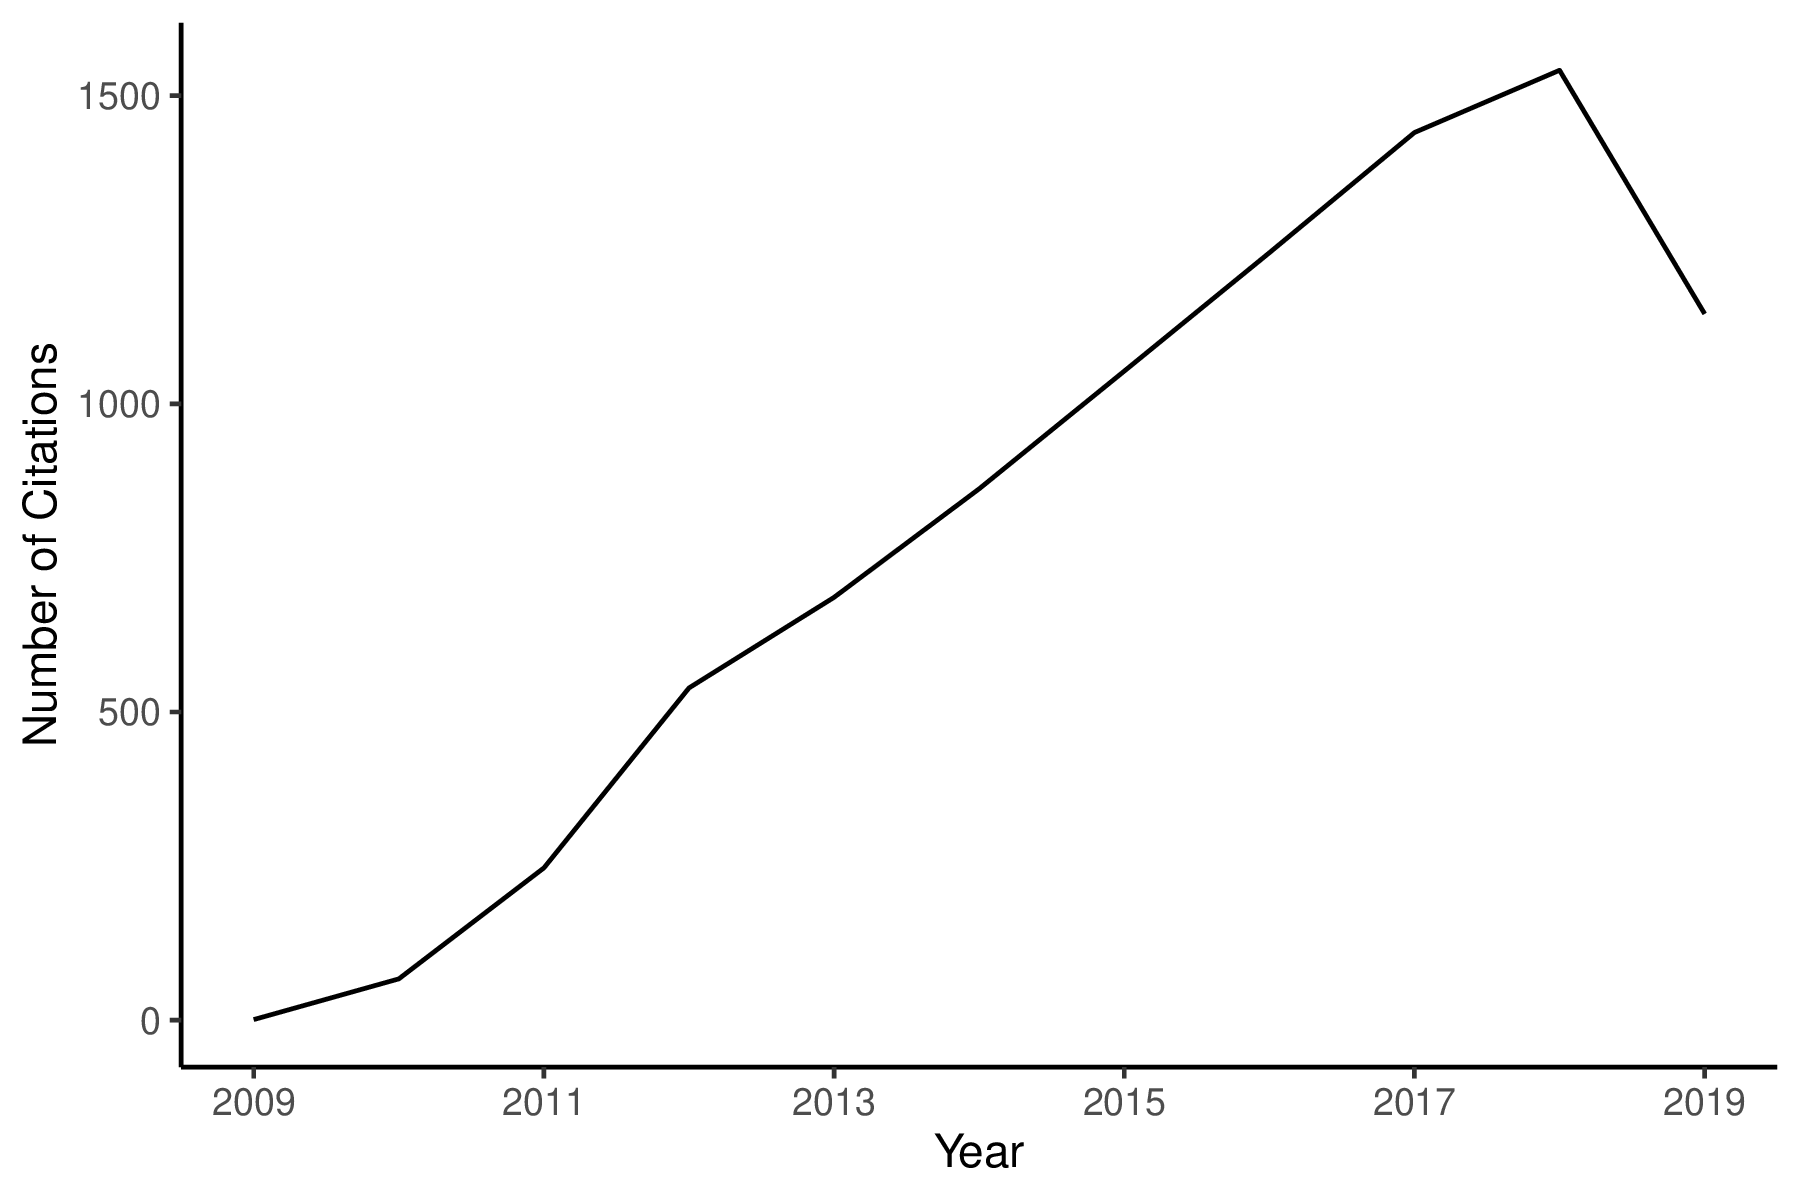
\includegraphics{figure_1.png}

\textbf{Figure 1. mothur has consistently been a popular software
package over the past ten years with more than 8,800 citations.}
Citation data taken from the Web of Science
(\url{https://www.webofscience.com}) on October 1, 2019. The gray line
segment depicts the projected number of citations for 2019 based on the
current number of citations for the year and historical trends.

\newpage


\includegraphics{figure_2.png}

\textbf{Figure 2. The mothur homepage.} From the mothur home page at
www.mothur.org, users can download mothur, access a user forum, navigate
a wiki with extensive documentation, find blog posts that provide
additional examples of how to use mothur, join the mothur facebook
group, and subscribe to the mothur mailing list.

\newpage


\includegraphics{figure_3.png}

\textbf{Figure 3. The start up window when running mothur in Mac OS X in
the interactive mode.} mothur can also be run on Windows or Linux. In
the interactive mode users enter individual commands at the mothur
prompt. Alternatively, users may run mothur by supplying commands from
the command line or using batch scripts.


\end{document}
